\documentclass[../../syllabus_1.tex]{subfiles}
\begin{document}



\chapter{Addition et soustraction d'entiers}

\section*{Matières}
\begin{enumerate}[label=\textbf{\arabic*.}]
    \item L’ensemble des nombres entiers.
    \item Opposés et valeur absolue.
    \item Addition et soustraction d’entiers.
    \item Règle des signes successifs.
    \item Positionnement sur une droite graduée.
    \item Comparaison de nombres entiers.
\end{enumerate}

\section{Les nombres négatifs et la valeur absolue : nous, on n'a pas peur!}
Aujourd'hui, personne ne s'étonne de voir un nombre comme \(-5 \). Pourtant, pendant très longtemps, les mathématiciens ont refusé d'utiliser les nombres négatifs ! Imaginez un marchand du Moyen Âge. Il possède \(7\) pièces d'or, mais il doit en rembourser \(10\). Combien lui reste-t-il ? Aujourd'hui, nous répondrions facilement : il a \(-3\) pièces, c'est-à-dire une dette de \(3\) pièces. Mais à l'époque, beaucoup de savants trouvaient cette réponse absurde.

Au XVIe siècle, certains mathématiciens appelaient même les nombres négatifs des « nombres faux » ou « absurdes ». Comment un nombre pourrait-il être plus petit que rien ? On pouvait compter des moutons, des pommes ou des pièces d'or, mais comment compter « moins trois pommes » ?

Même le grand mathématicien René Descartes parlait parfois des solutions négatives comme de solutions « fausses ». Il a fallu plusieurs siècles pour que les mathématiciens acceptent que ces nombres représentent autre chose que des objets : des dettes, des déplacements, des températures, des gains et des pertes.

Mais au fait, pourquoi les nombres négatifs sont-ils utiles ? Les nombres négatifs apparaissent partout autour de nous.
En hiver, la température peut descendre à \(-5\) °C.
Sur un compte bancaire, un solde de \(-20\) € signifie que l'on doit \(20\) €.
Dans un ascenseur, certains parkings sont au niveau \(-1\) ou \(-2\).
En montagne ou en plongée, on peut mesurer des altitudes ou des profondeurs négatives.
Dans les jeux vidéo ou les compétitions, on peut gagner ou perdre des points.

Les nombres négatifs permettent donc de représenter des situations où l'on est en dessous d'une référence : en dessous de zéro, en dessous du niveau de la mer, ou en dette.

Et la valeur absolue alors, qu'est-ce que c'est ?
Pour comparer des nombres négatifs, les mathématiciens ont inventé une idée très simple : la distance à zéro.

Par exemple :

\(|5| = 5 \)

\(|-5| = 5 \)

La valeur absolue ne regarde pas le signe ; elle mesure seulement l'éloignement par rapport à zéro.

C'est comme si l'on demandait : « À quelle distance suis-je du point de départ ? »

Que l'on fasse \(5\) pas vers la droite ou \(5\) pas vers la gauche, on est toujours à une distance de 5 pas du départ.


\section{Découverte des nombres entiers}

Voici plusieurs images de thermomètres.
\begin{center}
    
\includegraphics[width=.75\linewidth]{chapitres/addition_et_soustraction_avec_les_nombres_entiers/figures/thermo_v2.png}
\end{center}

\begin{enumerate}
    \item Sur quel thermomètre la température est-elle la plus froide ? La plus chaude ?\vspace*{2cm}
    \item Place ces températures sur une droite graduée.

        %   \includegraphics[width=\linewidth]{chapitres/addition_et_soustraction_avec_les_nombres_entiers/figures/droite_graduee_-20_40.tikz}
\end{enumerate}
\vspace{3cm}

\section{Un nouvel ensemble : les entiers}
\subsection{Vocabulaire}

Quels nouveaux nombres viens-tu de rencontrer ? 

Aux nombres naturels viennent s'ajouter ces nombres pour former un nouvel ensemble qui se note : 
\vspace{0.5cm}

Graphiquement, ces deux ensembles de nombres peuvent se représenter de la manière suivante : 
\vspace{5cm}

Cela signifie que tous les nombres naturels sont des nombres entiers. Mais l'inverse n'est pas vrai! Tout les nombres entiers ne sont pas des nombres naturels. Par exemple,

\newpage
\subsection{L'abscisse d'un point}

Lorsque l'on repère un point sur une droite graduée, on le repère grâce à un nombre, appelé dans ce contexte l'abscisse du point. Attention, elle n'est pas toujours un nombre entier.

Par exemple, le point $F$ sur la droite graduée suivante a comme abscisse $3$ qui sera notée $abs~F = 3$ ou $F(3)$.

\begin{center}
    \begin{tikzpicture}[scale=1.3]
        \draw[->] (-0.7,0) -- (8.7,0);
        \foreach \i in {0,...,8} {
            \draw (\i,0.1) -- (\i,-0.1);
            \node[below] at (\i,-0.3) {$\i$};
        }
        \filldraw (0,0) circle (2pt) node[above=3pt]{$N$};
        \filldraw (3,0) circle (2pt) node[above=3pt]{$F$};
        \filldraw (4,0) circle (2pt) node[above=3pt]{$A$};
        \filldraw (8,0) circle (2pt) node[above=3pt]{$T$};
    \end{tikzpicture}
\end{center}

Donne l'abscisse des points suivants.

\begin{enumerate}[cols=3, label=]
    \item $abs~A=$
    \item $abs~T=$
    \item $abs~N = $
\end{enumerate}

\begin{exercise}
    Place sur la droite graduée suivante les points dont voici les abscisses.
    \begin{enumerate}[cols=3, label=]
        \item $abs~C=0 $
        \item $abs~D= -2$
        \item $abs~E= 6$
        \item $abs~F= 5$
        \item $abs~X= -1$
        \item $abs~Y= 4$
    \end{enumerate}
    \begin{center}
        \begin{tikzpicture}[scale=1]
            \draw[->] (-3.7,0) -- (6.7,0);
            \foreach \i in {-3,...,6} {
                \draw (\i,0.1) -- (\i,-0.1);
                \node[below] at (\i,-0.3) {$\i$};
            }
        \end{tikzpicture}
    \end{center}
\end{exercise}

\begin{exercise}
    Donne l'abscisse des points suivants.
    \begin{center}
        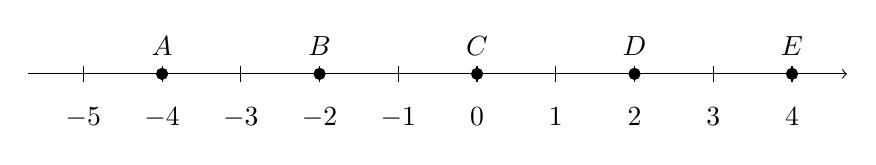
\begin{tikzpicture}[scale=1]
            \draw[->] (-5.7,0) -- (4.7,0);
            \foreach \i in {-5,...,4} {
                \draw (\i,0.1) -- (\i,-0.1);
                \node[below] at (\i,-0.3) {$\i$};
            }
            \filldraw (-4,0) circle (2pt) node[above=3pt]{$A$};
            \filldraw (-2,0) circle (2pt) node[above=3pt]{$B$};
            \filldraw (0,0)  circle (2pt) node[above=3pt]{$C$};
            \filldraw (2,0)  circle (2pt) node[above=3pt]{$D$};
            \filldraw (4,0)  circle (2pt) node[above=3pt]{$E$};
        \end{tikzpicture}
    \end{center}
    \begin{enumerate}[cols=5, label=\ ]
        \item $abs~A= $
        \item $abs~B= $
        \item $abs~C= $
        \item $abs~D= $
        \item $abs~E= $
    \end{enumerate}
\end{exercise}

\subsection{Opposés et valeur absolue}
\dotsforanswer{3}[Qu'est ce que la valeur absolue d'un nombre?]


\includegraphics[]{chapitres/addition_et_soustraction_avec_les_nombres_entiers/figures/valeur absoluee.png}

\dotsforanswer{3}[Que sont deux nombres opposés?]

\begin{itemize}[label=$\bullet$, cols=2]
    \item L'opposé de 5 est \dotfill
    \item L'opposé de $-3$ est \dotfill
\end{itemize}

\begin{exercise}
    Décode.
    \begin{enumerate}[itemsep=1cm]
        \item $-9$ \dotfill
        \item $-\left(4+3\right)$ \dotfill
        \item $ 5 + (-3)$ \dotfill
    \end{enumerate}
    \vspace{1cm}
\end{exercise}

\begin{exercise}
    Comment note-t-on l'opposé de $-3$? \dotfill
\end{exercise}

\begin{exercise}
    Complète les égalités suivantes.
    \begin{enumerate}[cols=3, itemsep=1em]
        \item $|-5|=$
        \item $|7|=$
        \item $|12|=$
        \item $|-12|=$
        \item $-|12|=$
        \item $-|-12|=$
    \end{enumerate}
\end{exercise}

\begin{exercise}
    Cite
    \begin{enumerate}[itemsep=1em]
        \item deux nombres de signes contraires qui ne sont pas opposés \dotfill
        \item deux nombres distincts ayant la même valeur absolue \dotfill
        \item deux nombres opposés dont la valeur absolue est inférieure à 3 \dotfill
        \item un nombre inférieur à 2 dont la valeur absolue est supérieur à 10 \dotfill
    \end{enumerate}
\end{exercise}

\newpage
\subsection{Comparaison de deux nombres entiers}
\begin{enumerate}[label=\arabic*), itemsep=1em]
    \item De deux nombres positifs, le plus petit est celui qui a la plus petite valeur absolue.
    \item De deux nombres négatifs, le plus petit est celui qui a la plus grande valeur absolue.
    \item De deux nombres de signes contraires, le plus petit est le nombre négatif.
\end{enumerate}

\begin{exercise}
    \begin{enumerate}[itemsep=2em]
        \item Quel est le plus petit nombre entier que tu peux écrire à l'aide des chiffres 2, 4, 8 et 0 ?
        \item Quel est le plus petit nombre naturel que tu peux écrire à l'aide des chiffres 2, 4, 8 et 0?\item Quel est le plus grand nombre entier que tu peux écrire à l'aide des chiffres 2, 4, 8 et 0 ?
    \end{enumerate}
    \vspace*{2em}
\end{exercise}

\begin{exercise}
    Compare les entiers suivants. Utilise les signes <, > ou =.

    $\begin{tblr}{colspec={cccXcccXccc}, rows={1cm}}
            -3 & \dots & -2 &  & 10  & \dots & -17 &  & -2 & \dots& -40 \\
            8  & \dots & 9  &  & -25 & \dots & -30 &  & 0  & \dots& -7
        \end{tblr}$
\end{exercise}


\newpage
\section{Addition et soustraction d'entiers }
\subsection{Somme de deux termes}
\setcounter{exercise}{0}
Pierre-Yves participe à un jeu de hasard. Il se joue en deux manches : à chaque manche, un gain ou une perte d'argent est noté.

\begin{enumerate}
    \item Donne le bilan de chacune des parties suivantes en écrivant l'opération à effectuer.
          \begin{enumerate}[itemsep=2em, label=\ ]
              \item Partie 1 : Pierre-Yves a gagné 3 € puis a gagné 7 €. Bilan : \dotfill
              \item Partie 2 : Pierre-Yves a gagné 8 € puis a perdu 5 €. Bilan : \dotfill
              \item Partie 3 : Pierre-Yves a perdu 4 € puis a gagné 8 €. Bilan : \dotfill
              \item Partie 4 : Pierre-Yves a perdu 9 € puis a perdu 2 €. Bilan : \dotfill
          \end{enumerate}
          \vspace{2em}
    \item Juan a rejoint Pierre-Yves et a noté ses propres résultats dans un tableau. Complète la dernière colonne.
          \begin{center}
              \begin{tblr}{
                      hlines,
                      vlines,
                      columns={2cm, c},
                      rows={1cm,m},
                      row{1}={gray!40, font=\bfseries},
                      column{1}={gray!40, font=\bfseries},
                  }
                  Partie n° & 1ère manche & 2ème manche & Bilan de la partie \\
                  1         & +4          & +7          &                    \\
                  2         & +9          & -5          &                    \\
                  3         & -4          & -6          &                    \\
                  4         & -9          & +2          &                    \\
                  5         & -7          & +10         &                    \\
                  6         & +5          & -7          &                    \\
                  7         & -7          & -11         &                    \\
              \end{tblr}
          \end{center}
          \vspace{1em}
    \item \dotsforanswer{2}[Au total, Juan aura-t-il perdu ou gagné de l'argent? Laisse ton calcul visible. ]
\end{enumerate}

\newpage
En te basant sur tes observations de la page précédente, réponds aux questions suivantes~:

\begin{itemize}[label=$\bullet$]
    \item \dotsforanswer{4}[Comment fait-on pour additionner deux nombres entiers de même signe?]
          \begin{enumerate}[itemsep=1cm, label=\ , cols=2]
              \item $\left(-6\right) + \left(-3\right)=$
              \item $10 + 4=$
              \item $-5 + (-3)=$
              \item $+7 + (+8)=$
          \end{enumerate}
          \vspace{1cm}
    \item \dotsforanswer{4}[Comment fait-on pour additionner deux nombres entiers de signes différents?]
          \begin{enumerate}[itemsep=1cm, label=\ , cols=2]
              \item $\left(-6\right) + \left(+13\right)=$
              \item $\left(+7\right) + \left(-12\right)=$
              \item $(-5)+20=$
              \item $27 +(-7)=$
          \end{enumerate}
          \vspace{1cm}
\end{itemize}
\emph{Note : On ne peut jamais écrire deux signes consécutifs. C'est pourquoi nous mettons les signes concernés entre parenthèses !}

\begin{exercise}
    Effectue.
    \begin{enumerate}[cols=2, itemsep=1.5em]
        \item $( + 3) + ( + 9) =$
        \item $( - 5) + ( + 14)=$
        \item $( - 4) + ( - 6) =$
        \item $( + 7) + ( - 8) =$
        \item $( - 8) + ( - 15) =$
        \item $( + 13) + ( - 8) =$
    \end{enumerate}
\end{exercise}

\newpage
\subsection{Règle des signes successifs}

Écris les calculs suivants sans parenthèses, sans calculer le résultat. Attention, les résultats doivent être égaux de chaque côté de l'égalité~!
\begin{enumerate}[cols=2, itemsep=2em]
    \item $( + 3) + ( - 2) =$
    \item $( + 4) + ( + 7) =$
    \item $( - 5) + ( - 8) =$
    \item $( + 8) + ( - 9) =$
    \item $( - 9) - ( - 7) =$
    \item $(-4)-(-1)=$
    \item $( + 3) - ( + 8) =$
    \item $( - 10) - ( - 4) =$
\end{enumerate}
\vspace{1cm}

\begin{itemize}[label=$\bullet$]
    \item \dotsforanswer{3}[Si les signes successifs sont identiques, ]
          \begin{enumerate}[cols=2, itemsep=1cm, label=\ ]
              \item $\left(+6\right) - \left(-3\right)=$
              \item $10 + (+4)=$
              \item $8 + \left(+3\right)=$
              \item $-7 - (-19)=$
                    \vspace{1cm}
          \end{enumerate}
          \vfil
    \item \dotsforanswer{3}[Si les signes successifs sont différents, ]
          \begin{enumerate}[cols=2, itemsep=1cm, label=\ ]
              \item $\left(-6\right) + \left(-13\right)=$
              \item $\left(+7\right) - \left(+10\right)=$
              \item $8 + \left(-3\right)=$
              \item $-7 - (+19)=$
                    \vspace{1cm}
          \end{enumerate}
\end{itemize}

\newpage
\begin{exercise}
    Écris les calculs suivants sans parenthèses en t'aidant de la règle des signes successifs, puis effectue comme dans l'exemple. \\
    Exemple :
    \begin{align*}
        (+9)-(+7)+(+11) & = 9 - 7 + 11 \\
                        & =13
    \end{align*}
    \vspace{1em}

    \begin{enumerate}[itemsep=3cm, cols=2]
        \item $( + 4) - ( + 15) =$
        \item $( - 12) + ( - 5) =$
        \item $( - 10) - ( - 7) =$
        \item $14 - ( - 4) =$
        \item $( + 6) - ( + 6) =$
        \item $- 16 - ( + 4) + ( + 7) =$
        \item $4- ( - 1) + ( - 8) - ( + 7) =$
        \item $- 13 + ( - 6) + ( + 5) + ( - 9) =$
    \end{enumerate}
\end{exercise}

\vfil

\begin{exercise}
    Sacha et Samuel vont à la fête foraine. Ils misent la même somme d'argent au début d'un jeu. Sacha gagne 6€ puis perd 1,30€. Samuel perd 3,20€ puis gagne 7,10€. Lequel des deux amis a remporté le plus d'argent à la fin ? Laisse ta démarche visible.
\end{exercise}

\newpage
\begin{exercise}
    Complète la pyramide suivante en sachant que le nombre contenu dans une brique est la somme des deux nombres contenus dans les briques situées en-dessous d'elle.
    \begin{center}
        
\includegraphics[]{chapitres/addition_et_soustraction_avec_les_nombres_entiers/figures/pyramide.png}
    \end{center}
\end{exercise}

\begin{exercise}
    Sabrine a eu bien froid cette nuit. La radio annonce que la température est remontée de $5\degres C$ ce matin, et il fait actuellement $3\degres C$. Quelle était la température cette nuit?
    \vspace{2cm}
\end{exercise}

\begin{exercise}
    Effectue la somme de plusieurs nombres opposés. Que remarques-tu~? \\ Écris la propriété qui en découle.
    \vspace{5cm}
\end{exercise}

\begin{exercise}
    Calcule la valeur numérique de $a+b-c$ si $a=-3$, $b=-5$ et $c=-2$.
\end{exercise}

\newpage
\begin{exercise}
    Complète le tableau en calculant la valeur numérique des expressions suivantes.
    \begin{center}
        \begin{tblr}{
                hlines,
                vlines,
                columns={5cm, c},
                rows={4cm,m},
                row{1}={1cm, gray!40, font=\bfseries},
                column{1}={1cm, gray!40, font=\bfseries},
                column{2}={1cm, gray!40, font=\bfseries},
                column{3}={1cm, gray!40, font=\bfseries},
            }
            $a$ & $b$ & $c$ & $a+b-c$ & $a-(b+c)$ \\
            10  & -3  & 8   &         &           \\
            -6  & -5  & 2   &         &           \\
            3   & -8  & -2  &         &           \\
            7   & -2  & -5  &         &           \\
        \end{tblr}
    \end{center}
\end{exercise}

\newpage
\section{Exercices mélangés}
\setcounter{exercise}{0}

\begin{exercise}
    Donne le nombre opposé de chaque nombre ci-dessous.
    \begin{enumerate}[cols=3]
        \item -5
        \item 2
        \item -7
        \item 18
        \item -100
        \item 8
    \end{enumerate}
\end{exercise}

\begin{exercise}
    Donne la valeur absolue des expressions suivantes.
    \begin{enumerate}[cols=3]
        \item $|-5|$
        \item $-|-2|$
        \item $|3|$
        \item $|-9|$
        \item $|-6|$
        \item $-|-1|$
    \end{enumerate}
\end{exercise}

 \begin{exercise}
     Place les élements suivants sur une droite graduée en graduant de sorte que $1cm = 1$ unité. \\

     $\hfil abs~A = 3 \hfil abs~B=-2 \hfil abs~C=-1 \hfil abs~D=2 \hfil abs~E=5$
 \end{exercise}

 \begin{exercise}
    Place les élements suivants sur une droite graduée en graduant de sorte que $5cm = 1$ unité. \\
    
    $\hfil abs~F = -0,5 \hfil abs~G=-0,2 \hfil abs~H=1,4 \hfil abs~D=0 \hfil abs~E=-0,8$
\end{exercise}

\begin{exercise}
    Compare les nombres suivants. Utilise <, > ou =. \emph{(sur cette feuille)}
    \begin{enumerate}[cols=3, label=\ ]
        \item $-4 \ldots -5$
        \item $7\ldots-3$
        \item $-40\ldots-35$
        \item $10\ldots 13$
        \item $-2\ldots-3$
        \item $-14\ldots-13,5$
        \item $-7\ldots-27$
        \item $4\ldots 3$
        \item $-5 \ldots -10$
              %\FIXME: aligner les pointillés
    \end{enumerate}
\end{exercise}

\begin{exercise}
    Effectue.
    \begin{enumerate}[cols=3]
        \item $-3+7$
        \item $-9+15$
        \item $50-80$
        \item $3-7+2$
        \item $18+9-13$
        \item $50-1-71$
        \item $-15 +13 +12$
        \item $-6 -4 +7$
        \item $-5 + 5$
        \item $8 - 10 + 6$
        \item $10-15+2$
        \item $-50-17$
        \item $3-10+7$
        \item $7 + 8 - 20$
        \item $-7 -20$
    \end{enumerate}
\end{exercise}

\newpage
\begin{exercise}
    Effectue. Laisse tes étapes visibles.
    \begin{enumerate}[cols=3]
        \item $(-7)+(-10)$
        \item $( + 7) + ( - 10)$
        \item $25 - ( + 7)$
        \item $-50+(-2)-(-9)$
        \item $-2+5-(-7)$
        \item $14-(-5)+(-7)-(+10)$
        \item $12 + 7 - 25 + 3$
        \item $10 + ( - 7) - ( - 15)$
        \item $- 14 + 7$
        \item $( - 5) + ( + 8) - ( + 9)$
        \item $14 - ( - 7) + 17 - 28 - 5$
        \item $( - 5) + ( - 4) - ( - 12)$
        \item $- 5 + ( - 7) - ( + 8)$
        \item $- 12 - 13 - 14 + 15$
        \item $(-3)- (-5) - 10$
    \end{enumerate}
\end{exercise}

\begin{exercise}
    Calcule la valeur numérique des expressions suivantes. Laisse tes étapes visibles.
    \begin{enumerate}[cols=2, itemsep=1em]
        \item $x + y$ si $x=30$ et $y=-2$
        \item $a + b - c$ si $a=-1$, $b = -3$ et $c = -2$
        \item $10 + t - g$ si $t = -10$ et $g=4$
        \item $w - 7 + z$ si $w = 2$ et $z = -13$
        \item $p + o - p$ si $p = -3$ et $o = -5$
        \item $d + 5 - 7 + v$ si $d = -9$ et $v = 10$
        \item $5 + f + h$ si $f = -8$ et $h = -10$
        \item $a + 10 - b + c $ si $a = -7$, $b = -7$ et $c=2$
    \end{enumerate}
\end{exercise}

\newpage
\begin{exercise}
    Le professeur Mr Mathix donne à ses élèves un questionnaire à choix multiples (QCM) comportant huit questions. Il note de la façon suivante :
    \begin{center}
        \begin{minipage}{7cm}
            Réponse fausse (F) : -3 points \\
            Sans réponse (S) : -1 point \\
            Réponse correcte (B) : +4 points
        \end{minipage}
    \end{center}
    \begin{enumerate}
        \item Calcule la note de Logan dont les résultats aux questions sont F, B, S, F, F, B, B, S
        \item Quelle est la note la plus basse qu'un élève peut obtenir~? Et la plus haute~?
        \item Est-ce possible que Evelyne ait obtenu une note de 3 ? Laisse ton développement visible.
    \end{enumerate}
\end{exercise}

\begin{exercise}
    Voici une série de neuf nombres et des informations relatives à ceux-ci.\\ 

    1200 \hfil 0 \hfil -1355 \hfil -801 \hfil -1335 \hfil -600 \hfil 1448 \hfil 781 \hfil -1345  

    \begin{enumerate}[label=\ ]
        \item \(A\) est un nombre compris entre \(- 700\) et \(0\).
        \item \(E\) est le plus grand nombre de la série.
        \item \(G\) est l'abscisse de l'origine du repère sur une droite graduée.
        \item \(H\) est un nombre strictement négatif multiple de \(9\).
        \item \(O\) est un nombre qui est à la même distance de zéro que \(- 781\).
        \item \(P\) est le plus petit nombre de la série.
        \item \(R\) est un nombre strictement positif multiple de \(3\).
        \item \(T\) est un nombre négatif dont les chiffres des centaines et des dizaines sont les mêmes.
        \item \(Y\) est un nombre négatif plus petit que \(- 1340\) et plus grand que \(- 1356\).
    \end{enumerate}
    \begin{enumerate}
        \item Range les nombres proposés par ordre croissant.
        \item Associe chaque nombre de la série à la lettre correspondant à sa description.
        \item En t'aidant de la suite de nombres écrite au point \textbf{b)}, replace les lettres dans le bon ordre et découvre le nom d'un mathématicien connu.
    \end{enumerate}
\end{exercise}

\begin{exercise}
    Code/décode.
    \begin{enumerate}[cols=2]
        \item L'opposé de 7
        \item La somme de 8 et de l'opposé de 10 vaut l'opposé de 2
        \item La différence entre l'opposé de 6 et l'opposé de 7
        \item $-8+2=-6$
        \item $-5$
        \item $(-4)^2$
        \item $-4^2$
        \item $-3+3^3=24$
    \end{enumerate}
\end{exercise}

\newpage
\begin{exercise}
    Place les points suivants sur une droite que tu gradueras de sorte que \emph{2cm = 1 unité}.
    \begin{enumerate}[label=\ ]
        \item $A$ si tu sais que son abscisse vaut -3
        \item $B$ si tu sais que son abscisse vaut 0,5
        \item $C$ tel que $abs C = -2.5$
        \item $D$ si tu sais que son abscisse vaut la somme des abscisses de $B$ et $C$
        \item $E$ si tu sais que son abscisse vaut 3,5
        \item $F$ si tu sais que les abscisses de $E$ et $F$ sont des nombres opposés.
    \end{enumerate}
\end{exercise}

\begin{exercise}
    Complète le Minion dont voici le corps au centre en résolvant chacune des questions concernant ses cheveux, ses yeux, ses bras, ses pieds, sa tenue et sa bouche. \\ \emph{(Sur celle feuille)}
    \begin{center}
        
\includegraphics[]{chapitres/addition_et_soustraction_avec_les_nombres_entiers/figures/minion1.png}
    \end{center}
\end{exercise}

\newpage
\section{Je me teste}
\faIcon{exclamation-triangle}~Cette partie doit être réalisée sur une feuille annexe.
\setcounter{exercise}{0}

\begin{exercise}
    Trace une droite graduée, que tu construis de manière à pourvoir placer les nombres entiers suivant : \(-15, -5 , 0, 10, 20 \).
\end{exercise}

\begin{exercise}
    Trace une droite graduée, que tu construis de manière à pourvoir placer les nombres entiers suivant : \(-15, -9 , 0, 6 \)
\end{exercise}

\begin{exercise}
    Calcule.
    \begin{enumerate}[cols=2]
        \item \((+4) + (+3) = \)
        \item \((-5) + (-2) = \)
        \item \((+7) + (-3) = \)
        \item \((-6) + (+8) = \)
        \item \((+9) - (+4) = \)
        \item \((+5) - (-2) = \)
        \item \((-4) - (+3) = \)
        \item \((-7) - (-5) = \)
        \item \((+2) + (-6) = \)
        \item \((-3) + (+10) = \)
    \end{enumerate}
\end{exercise}

\begin{exercise}
    Calcule.
    \begin{enumerate}[cols=2]
        \item \((-8) + (+5) = \)
        \item \((+12) + (-9) = \)
        \item \((-15) + (+7) = \)
        \item \((+18) - (+25) = \)
        \item \((-20) - (+6) = \)
        \item \((-14) - (-8) = \)
        \item \((+16) - (-9) = \)
        \item \((+5) + (-12) = \)
        \item \((-9) + (-11) = \)
        \item \((+30) - (+18) = \)
    \end{enumerate}
\end{exercise}

\begin{exercise}
    Trouve la valeur manquante pour que le calcul soit correct.
    \begin{enumerate}[cols=2]
        \item \(\dots + (+6) = 11 \)
        \item \((-4) + \dots = 3 \)
        \item \(\dots + (-7) = -12 \)
        \item \((+9) + \dots = 2 \)
        \item \(\dots - (+5) = -8 \)
        \item \((+4) - \dots = -3 \)
        \item \(\dots - (-6) = 2 \)
        \item \((-8) - \dots = -10 \)
    \end{enumerate}
\end{exercise}

\newpage
\begin{exercise}
    Les géographes utilisent une altitude de référence : le niveau de la mer, qui correspond à \(0\) m. Voici les altitudes et profondeurs de quelques lieux célèbres :
    \begin{center}
        \begin{tabular}{|l|r|}
            \hline
            \textbf{Lieu} & \textbf{Altitude / Profondeur} \\
            \hline
                Mont Blanc                                 & $+4\,810$ m  \\
                Tour Eiffel (sommet)                       & $+330$ m     \\
                Niveau de la mer                           & $0$ m        \\
                Épave du Titanic                           & $-3\,800$ m  \\
                Grand Canyon (fond de certaines gorges)    & $-1\,800$ m  \\                    Fosse des Mariannes                        & $-11\,000$ m \\
            \hline
        \end{tabular}
    \end{center}
    \begin{enumerate}
        \item Trace une droite graduée (verticale) et place chacun de ces lieux au bon endroit en choisissant une échelle adaptée. 
        \item Quels sont les lieux situés en-dessous du niveau de la mer ? 
        \item Quel est le lieu le plus élevé ? 
        \item Quel est le lieu le plus profond ?
        \item Classe ces lieux du plus bas au plus haut en utilisant des notations mathématiques adaptées.  
    \end{enumerate}
\end{exercise}

\newpage
\section*{Mots-clés}
\begin{enumerate}[cols=2, label=\textbf{\arabic*.}]
    \item Abscisse
    \item Nombres opposés
    \item Valeur absolue
    \item Nombres entiers
    \item 
\end{enumerate}

\section*{Attendus}
\begin{enumerate}[label=\textbf{\arabic*.}]
    \item Placer sur la droite graduée des nombres entiers positifs (naturels) et leurs opposés.
    \item Identifier un nombre naturel, un nombre entier.
    \item Associer l’expression « opposé d’un nombre » à son écriture mathématique et à sa représentation sur une droite graduée.
    \item Associer les symboles d’ordre ( <, >, = ) aux expressions « est plus petit que », « est plus grand que », « est égal à » et à leurs positions respectives sur une droite orientée graduée.
    \item Placer un nombre (naturel, entier) sur une droite graduée.
    \item Comparer deux nombres (entiers) en utilisant le symbole adéquat ( <, >, = ).
    \item Encadrer un nombre entier à l'unité, au dixième ou au centième près.
    \item Ordonner des nombres entiers par ordre croissant ou décroissant.
    \item Associer à l’addition et à la soustraction de deux nombres entiers un déplacement ou un écart sur la droite numérique.
    \item Calculer une somme et une différence de nombres entiers.
    \item Calculer en utilisant les propriétés des opérations (commutativité, associativité, neutre, absorbant) et la distributivité.
    \item Calculer en utilisant les priorités des opérations.
    \item Vérifier la plausibilité d’un résultat (cohérence avec l’estimation ou cohérence avec la situation).
    \item Utiliser la calculatrice pour vérifier le résultat d’une opération (nombres entiers).
\end{enumerate}

\end{document}